%% LyX 2.2.4 created this file.  For more info, see http://www.lyx.org/.
%% Do not edit unless you really know what you are doing.
\documentclass[english]{article}
\usepackage{lmodern}
\usepackage[T1]{fontenc}
\usepackage[latin9]{inputenc}
\usepackage{geometry}
\geometry{verbose,tmargin=3cm,bmargin=3cm,lmargin=2.5cm,rmargin=2.5cm}
\usepackage{textcomp}
\usepackage{graphicx}
%\usepackage{mcode}

\renewcommand\thesection{\alph{section}}

\makeatletter

%%%%%%%%%%%%%%%%%%%%%%%%%%%%%% LyX specific LaTeX commands.
%% Because html converters don't know tabularnewline
\providecommand{\tabularnewline}{\\}

\makeatother

\usepackage{babel}

\usepackage{pdfpages}
\usepackage{amsmath}
\usepackage{listings}

\begin{document}

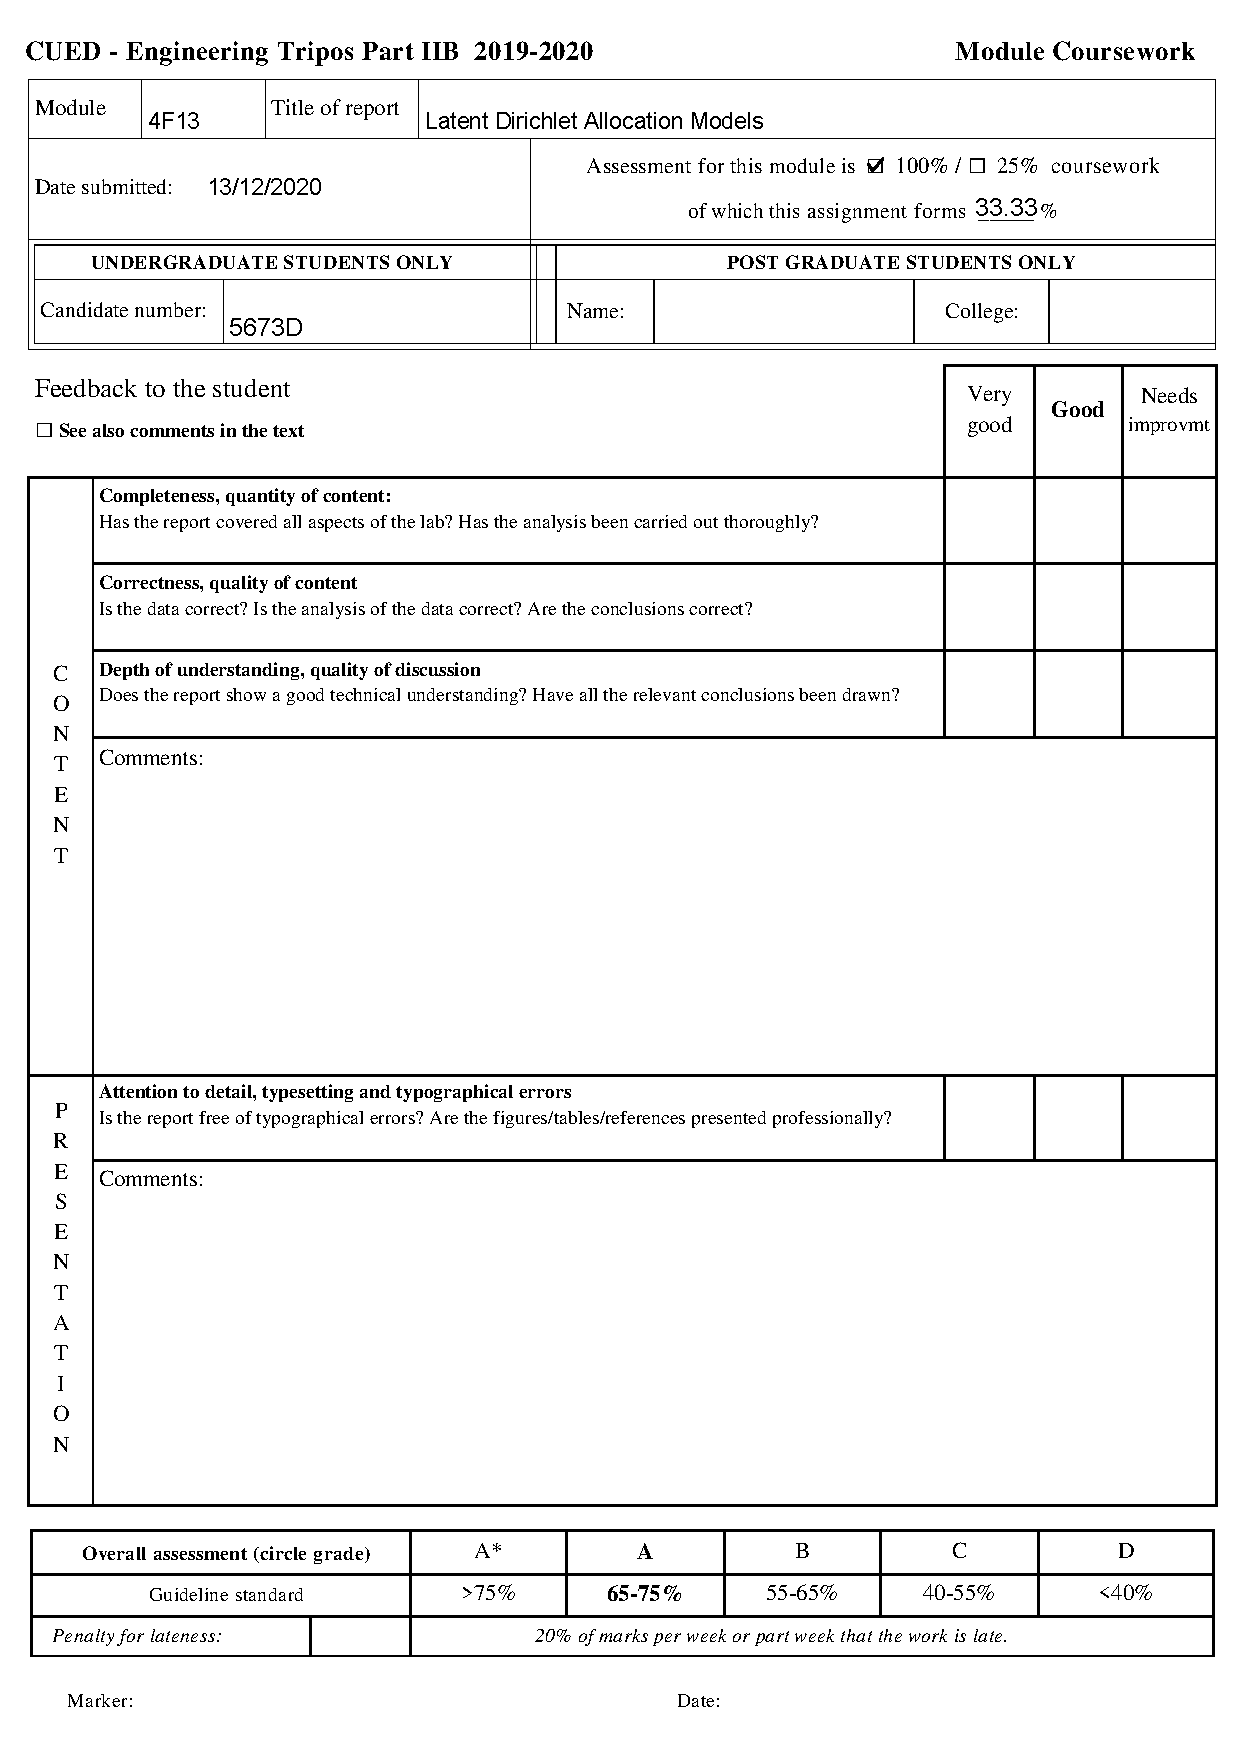
\includepdf{cover.pdf}
\title{4F13: Probabilistic Machine Learning\\
Latent Dirichlet Allocation model}

\author{Candidate number: 5673D \\
		Words count: approximetly 985
	}

\maketitle

\section{Maximum Likelihood Multinomial over Words \label{a}}
	
From the lecture notes, we already know that after maximising the likelihood we get the following form for the parameters $ \mathbf{\beta} $:

\begin{equation*}\label{1}
	\hat{\beta}_m = \frac{c_m}{N}
\end{equation*}	
where $ c_m $ is the total count of the world $ m $ in $ A $ and $ N $ is the total number of words in $ A $. In other words, $ \hat{\beta}_m $ is the normalised frequency of word $ m $. To find this values, we will use the following code:

\begin{verbatim}
load kos_doc_data.mat
	
W = max(A(:,2));                                     % number of unique words in A
D = max(A(:,1));                                     % number of document in A
word_frequency = zeros(W,1);                         % initialise frequency of each word
	
for i=1:size(A)                                      %iterate over entries
    w = A(i, 2);                                     %get the word in the entry
    c = A(i, 3);                                     % get the counts for the word 
    word_frequency(w,1) = word_frequency(w,1) + c;   %add the counts
end
	
word_frequency = word_frequency/sum(word_frequency); %normalise
\end{verbatim}

 

In this model, the probability of a word is equal to its frequency in the collection $ A $. This means that if a word appears in the test set $ B $ and it does not appear in the training set $ A $, its probability is equal to zero. If we calculate the log-probability of a new word, we get minus infinity. This shows us that this model cannot process new words. Moreover, any model that will give finite values for the log-probability will be better than this one. 

\newpage

\begin{figure}[h]
	\begin{centering}
		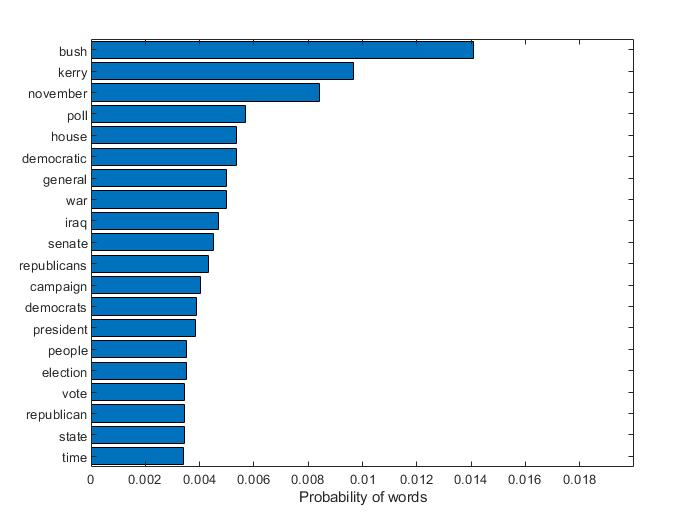
\includegraphics[width=0.3\paperwidth]{1a.jpg}\hspace{1cm}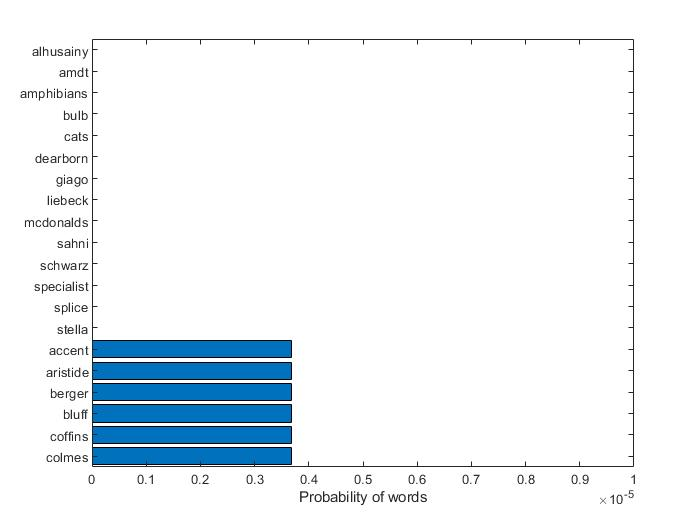
\includegraphics[width=0.3\paperwidth]{1b.jpg}
		\par\end{centering}
	\caption{ On the left: The most probable 20 words. On the right: The least probable 20 words.
		\label{fig:1} }
\end{figure}   

\section{Bayesian Inference using Symmetric Dirichlet prior \label{b}}

In this model we want to solve the problem of new words with zero probability. To do that we propose using Bayesian inference using a symmetric Direchlet prior with $ \alpha $ as a concentration parameter. Our new probability distribution over the words is:

\begin{equation*}
	p(w_m|\alpha, A)= \beta_m = \frac{c_m+\alpha}{\sum_{l=1}^{M}(c_l + \alpha)}
\end{equation*}

where the parameter $ \alpha $ acts as the pseudo-counts of each word and $ M $ is the size of the vocabulary. This model increases the probability of words with small frequencies and decreases the probability of the words with high frequency. For instance, if $ \alpha  = 1$ (small), the probability of words that appear once is increased by almost $ 100\% $, while the probability of common words is only slightly decreased. If $ \alpha = 10^6 $ (very large) our probability distribution tends to a uniform distribution, which is expected as the pseudo-counts become much larger than the actual counts.
   
\begin{verbatim}
	alpha = 1;                                                 %set the parameter
	word_frequency = word_frequency + alpha;                   %add the pseudo-counts
	bayes_word_frequency = word_frequency/sum(word_frequency); %normalise
\end{verbatim}

\begin{figure}[h]
	\begin{centering}
		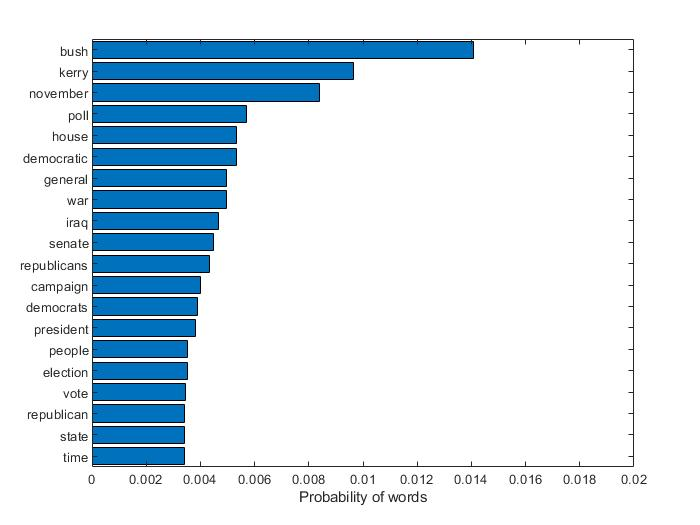
\includegraphics[width=0.3\paperwidth]{2a.jpg}\hspace{1cm}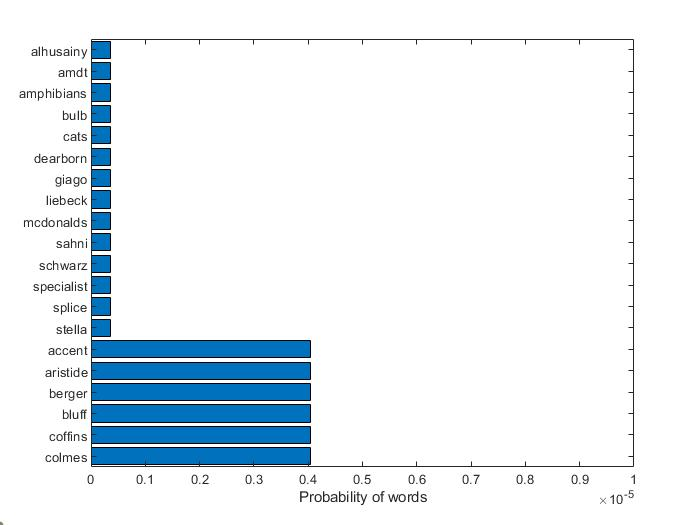
\includegraphics[width=0.3\paperwidth]{2b.jpg}
		\par\end{centering}
	\caption{ Using Bayesian inference:
		On the left: The most probable 20 words. On the right: The least probable 20 words.
		\label{fig:2} }
\end{figure}   

\section{Probabilities and perplexities of the test set}

In this section, we are interested in finding a measure of performance. To do this, we need will make use of the joint probability of a collection and per word perplexity.

The probability of a given sequence of words(document) is define as:

\begin{equation*}
	p(\mathbf{w}|\mathbf{\beta}) = \prod_{m=1}^{M} \beta_m^{c_m^{(test)}}
\end{equation*} 
where $ \beta_m $ is probability of appearance of word $ m $ and $ c_m^{(test)} $ is the word $ m $ count inside the test collection. Note that we are interested in a specific sequence(order) of words and we do not use the combinatorial factor. Therefore, this is a categorical distribution function. 
Taking the $ \log $ of the probability, we get:
\begin{equation*}
	\log(p(\mathbf{w}|\mathbf{\beta})) = \sum_{m=1}^{M}c_m^{(test)}\log(\beta_m)
\end{equation*}

The per word perplexity is given by:
\begin{equation*}
	Perpelexity = \exp\left(-\frac{p(\mathbf{w}|\mathbf{\beta})}{N}\right)
\end{equation*}
where $ N $ is the total number of counts.
The result for two documents in the test set $ B $ and over all documents in $ B $ are presented below. We used $ \beta $s found in section \ref{b} with $ \alpha=1$.
\begin{table}[h]
	\begin{center}
		\begin{tabular}{cc |c |c|c|c|}
			Document ID& Words count & Unique words & log probability & Perplexity\tabularnewline
			\cline{2-5} 
			2001 & 440 & 232 & -3688  & 4373\tabularnewline
			\cline{2-5} 
			2060 & 106 & 87 & -816  & 2222\tabularnewline
			\cline{2-5} 
			All documents & 195816 & 6870 & -1.54e-6 & 2683\tabularnewline
			\cline{2-5} 
		\end{tabular}
		\par\end{center}
	\caption{Log-Probabilities and perplexities\label{tab:3}}
\end{table}
    
The perplexity is a measure that defines the average uncertainty over the words. Therefore, we expect lower perplexities values for documents that has similar distributions to our training set $ A $ (see document $ 2060 $) and higher values for documents that have more uncommon words. The perplexity over all documents has a general lower value for perplexity because of the large number of words. The larger the number of words, the closer we are to the true distribution. 
In the case of uniform distribution over words: $ \beta_m = 1/M $. Therefore, $ \log(p) = -N_B\log(M) $ and the perplexity $ =M=6906 $.

\begin{verbatim}
for i=1:size_B(1)                                %iterate over entries
    wb = B(i,2);                                 %get word ID
    cb = B(i,3);                                 %get word count
    frequency_b = bayes_word_frequency(wb);      %get the word's frequency
    log_p = log_p + cb * log(frequency_b);       %recalculate the log-probability
    word_count = word_count + cb;                %add to the total word count
    if (B(i,1) == D_1)                           %do the same thing for a specific document
        log_p1 = log_p1 + cb * log(frequency_b);
        word_count1 = word_count1 + cb;
    end
end
\end{verbatim}

\section{Mixture of multinomials model}
In this section, we are interested in splitting our word in a number of topics $ K $. The mixing proportions are:
\begin{equation*}
	p(\theta|\mathbf{z}, \alpha) \propto Dir(\mathbf{c}+\alpha)
\end{equation*}
where $ c_k $ are the counts for mixture $ k $.
Now, if we keep track of this mixing proportions after each Gibbs step and normalise them using the code below:
\begin{verbatim}
mixing_prop(:,iter+1) = sk_docs + alpha;
mixing_prop(:,iter +1) = mixing_prop(:, iter +1)/ sum(mixing_prop(:, iter +1));
\end{verbatim}

We get the results in Fig. \ref{fig:3}. We can see that after almost 20 steps, the mixing proportions reach a plateau. This means they converged to a final value. Running the program multiple times, we observed that the final values are not always the same. This behaviour is explained by the initial random generated seeds that converge to a local maximum of the posterior. Once they reach a local minimum they cannot longer explore the whole space for the global maximum. A method to choose between this local maxima is to take the one with minimum perplexity.   

\begin{figure}[h]
	\begin{centering}
		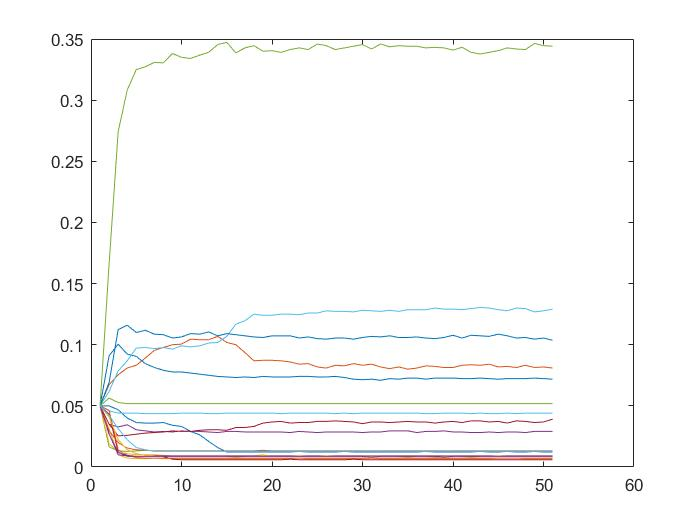
\includegraphics[width=0.3\paperwidth]{4a.jpg}\hspace{1cm}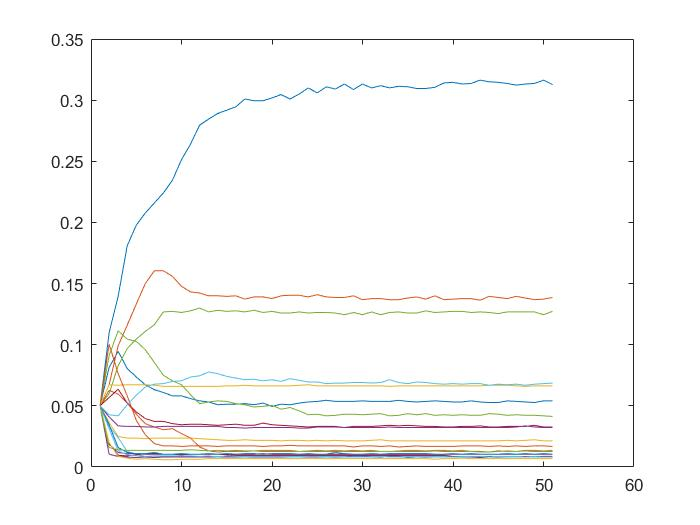
\includegraphics[width=0.3\paperwidth]{4b.jpg}
		\par\end{centering}
	\caption{ Mixing Proportions vs Gibbs iterations
		\label{fig:3} }
\end{figure}   

\section{Latent Dirichlet Allocation model}
Now, let us have a look at how Latent Dirichlet Allocation model performs in comparison with our previous approaches. By looking at the mixing proportion, we can see that we have more relevant topics than we previously had. Moreover, now we have more than one dominant topic. By comparing the perplexities for different models(See Table \ref{tab:4}), we can determine that this model has the lowest perplexity, although it does not seem to converge after $ 50 $ iterations. Moreover, increasing the number of iterations will result in a  marginally better perplexity, but will take considerately more time to compute. Depending on what we want to obtain(accurate prediction or computational speed), we can say that $ 50 $ iterations are a fairly good trade off between our targets.

\begin{table}[h]
	\begin{center}
		\begin{tabular}{cc |c |c|c|c|}
			Model& ML & BI & BMM & LDA\tabularnewline
			\cline{2-5} 
			Perplexity & -$\infty$ & 2683 & 2110  & 1647\tabularnewline
			\cline{2-5} 
		\end{tabular}
		\par\end{center}
	\caption{Log-Probabilities and perplexities\label{tab:4}}
\end{table}

The world entropy for each topic is given by the following formula:
 
\begin{equation*}
	H = -\sum_{m=1}^{M}p(w_m|A,\gamma,z=k) \log_2(p(w_m|A,\gamma,z=k)) bits
\end{equation*}

where $ p(w_m|A,\gamma,z=k) $ is the probability of the word $ m  $coming from the topic $ k $. The units used for the word entropy are bits. Again we plot this as entropy for each topic as function of the Gibbs iterations. We can see that the entropy of each topics decreases from the starting value(uniform distribution) as it becomes closer to the true distribution. This behaviour it is highly expected, as the entropy has its maximum when the distribution is uniform. The difference between mixing proportion and entropy is that the entropy converges faster( \~ 25 iterations) and after that there is little change in values. Also the more probable words and topics has the lowest entropy.

\begin{figure}[h]
	\begin{centering}
		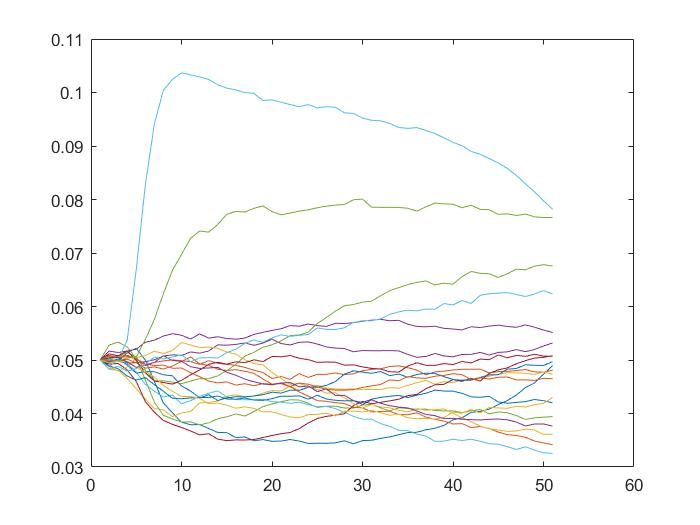
\includegraphics[width=0.3\paperwidth]{5a.jpg}\hspace{1cm}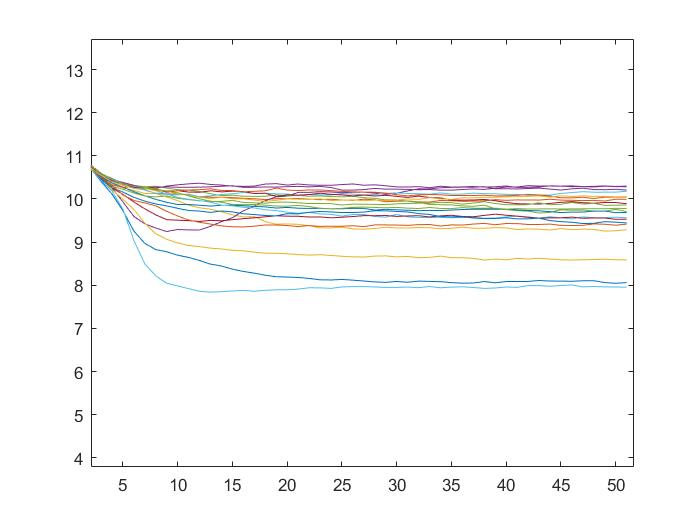
\includegraphics[width=0.3\paperwidth]{5b.jpg}
		\par\end{centering}
	\caption{ On the left: Mixing proportion vs Gibbs iteration. On the right: Word entropy vs Gibbs iterations
		\label{fig:5} }
\end{figure}   
\end{document}
